\documentclass{beamer}
\usetheme{Warsaw}
\setbeamertemplate{caption}[numbered]
\setbeamertemplate{navigation symbols}{}%remove navigation symbols

\usepackage{polski}
\usepackage[utf8]{inputenc}
\usepackage{array}
\usepackage{hyperref}
\usepackage{listings}

\title{Optymalizacja struktury sieci drogowej}
\author{Michał Siatkowski} 
\institute{Promotor: dr hab. inż. Aneta Poniszewska - Marańda \\
		Kopromotor: mgr inż. Łukasz Chomątek \\
		\vspace*{20px}
		Politechnika Łódzka}
\date{Łódź, FTIMS, Informatyka 2014/2015}

\begin{document}

\maketitle

\section{Wstep}
\subsection{Problematyka i zakres pracy}
\begin{frame}{Problematyka i zakres pracy} 

Niniejsza praca obejmuje zagadnienia z zakresu inżynierii oprogramowania i sztucznej inteligencji. Głównym jej celem jest stworzenie aplikacji optymalizującej strukturę sieci drogowej.

\end{frame}

\subsection{Cele pracy}
\begin{frame}{Cele pracy} 

Celami pracy są:
\begin{enumerate}

\item Zdefiniowanie problematyki optymalizacji struktury sieci drogowej.
\item Stworzenie aplikacji optymalizującej tę strukturę.
\item Analiza i ocena efektywności zastosowanych rozwiązań.

\end{enumerate}

\end{frame}

\subsection{Metoda badawcza}
\begin{frame}{Metoda badawcza} 
\newtheorem{mydef0}{Prototypowanie}
\begin{mydef0}
jest to proces budowy modelu matematycznego i obserwacja czy jego zachowanie może pomóc inżynierom w odkryciu ukrytych wad ich projektu. Z założenia prototypy nie wchodzą w skład ostatecznego systemu.
\end{mydef0}
\end{frame}

\subsection{Przeglad literatury w dziedzinie}
\begin{frame}{Przeglad literatury w dziedzinie} 

\begin{enumerate}

\item {
Wataru Nanya, Hiroshi Kitada, Azusa Hara, Yukiko Wakita, Tatsuhiro Tamaki, and Eisuke Kita\\
\emph{Road Network Optimization for Increasing Traffic Flow}. \\
Int. Conference on Simulation Technology, JSST 2013.}

\end{enumerate}
\end{frame}


\section{Optymalizacja struktury sieci drogowej}
\subsection{Podstawowe definicje}
\begin{frame}{Podstawowe definicje} 

\newtheorem{mydef1}{Sieć drogowa}
\begin{mydef1}
	\begin{figure}[h!]
	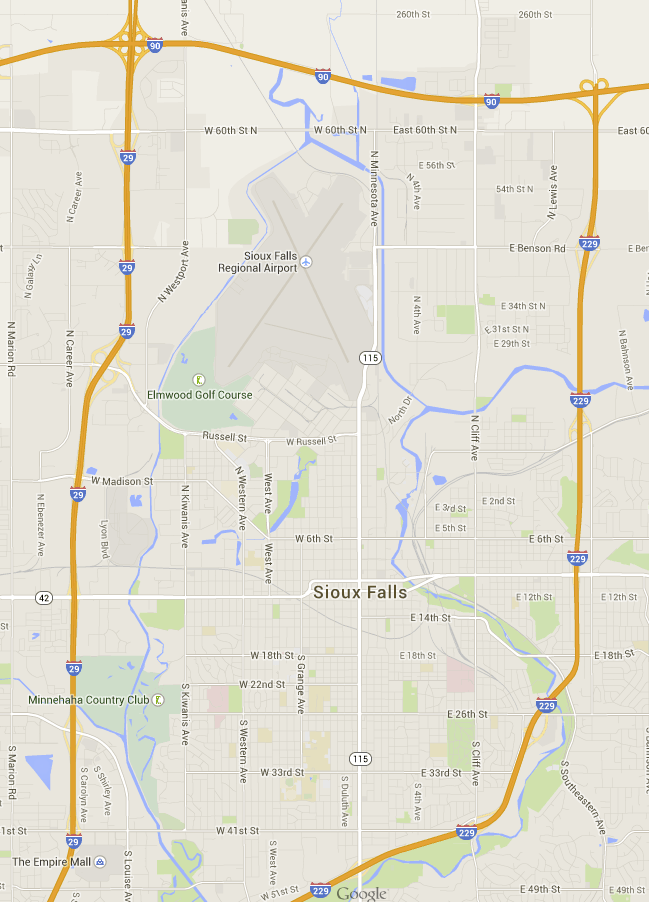
\includegraphics[width=0.30\textwidth]{img/siec}
	\caption{Fragment sieci drogowej w Sioux Falls, Południowa Dakota.} 
	\end{figure}
\end{mydef1}

\end{frame}

\begin{frame}{Podstawowe definicje} 

\newtheorem{mydef2}{Sieć drogowa w postaci grafu}
\begin{mydef2}
	\begin{figure}[h!]
	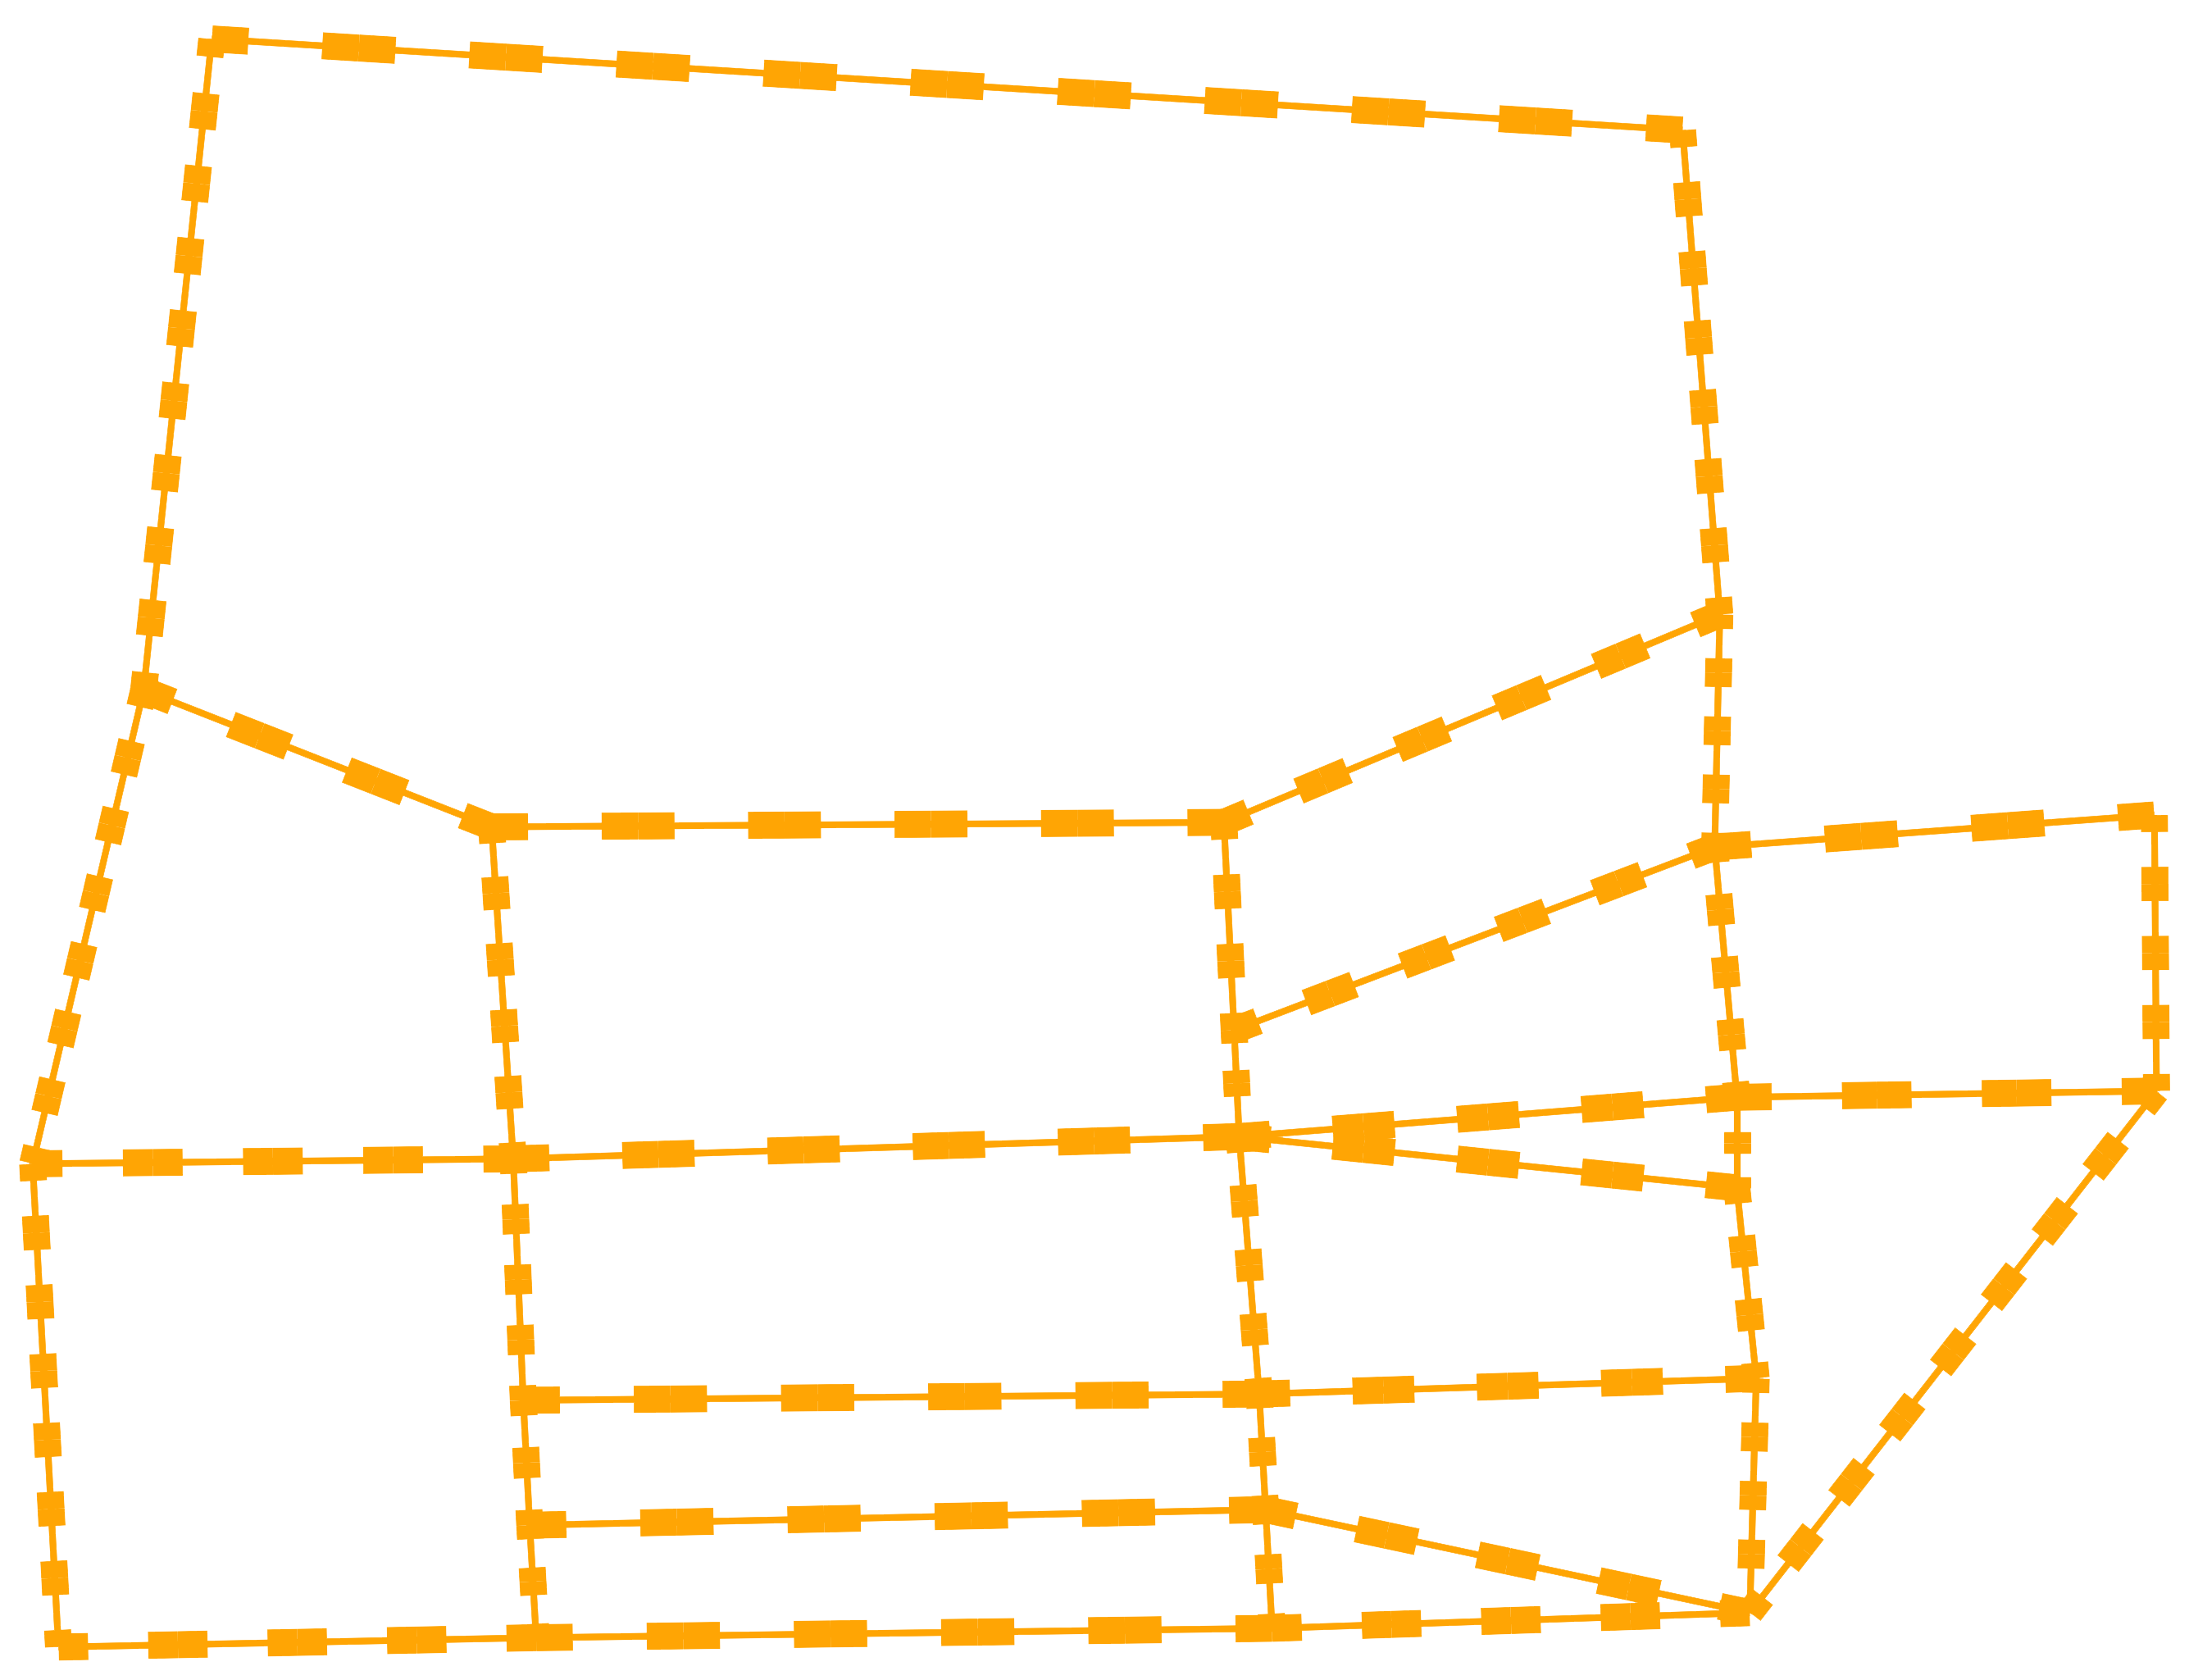
\includegraphics[width=0.55\textwidth]{img/graf}
	\caption{Siec drogowa miasta Sioux Falls w postaci grafu.} 
	\end{figure}
\end{mydef2}

\end{frame}

\begin{frame}{Podstawowe definicje} 
	\begin{figure}[h!]
	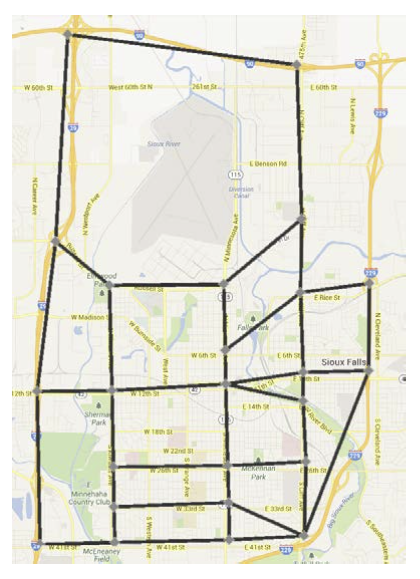
\includegraphics[width=0.38\textwidth]{img/dopasowanie}
	\caption{Graf z dopasowaną geometrią \cite{siux}.}
	\end{figure}
\end{frame}


\subsection{Paradoks Braessa }
\begin{frame}{Paradoks Braessa\cite{braess}}

\centering
\begin{minipage}{.48\textwidth}
\begin{figure}[h!]
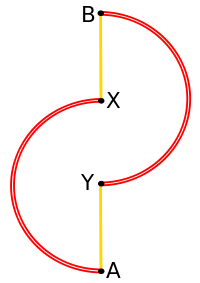
\includegraphics[width=0.7\textwidth]{img/braess1}
\caption{Wyjściowy układ drogowy}
\end{figure}
\end{minipage}\hfill
\begin{minipage}{.48\textwidth}

Autostrady:\\
AX, $t_{AX}(p) =  50 + p$ min\\
YB, $t_{YB}(p) =  50 + p$ min\\

Drogi lokalne:\\
AY, $t_{AY}(p) =  10p$ min\\
XB, $t_{XB}(p) =  10p$ min\\
\\
Aut jest 6000 i wszystkie mają za zadanie przejechać trasę z A do B.

\end{minipage}\hfill

\end{frame}


\begin{frame}{Równowaga Nasha\cite{braess}} 

Równowaga Nasha to taka sytuacja, w której każdy z samochodów spowoduje wydłużenie swojego czasu jazdy, zmieniając decyzję co do wyboru trasy przy niezmienionych decyzjach pozostałych aut.
\newline\newline
Jeśli p i q to liczby aut w tysiącach pokonujących odpowiednio trasy AXB i AYB, otrzymujmy równania:

\begin{center}
$p+q = 6 $\\
$t_{AX}(p)+t_{XB}(p) = t_{AY}(q) + t_{YB}(q)$\\
$50+p+10p = 10q+50+q$
\end{center}
rozwiązaniem jest $p=q=3$.\\
Przy tej gęstości ruchu pokonanie obu dostępnych tras zabiera $50+3+30=83$ minuty.
\end{frame}

\begin{frame}{Uzupełniony układ drogowy \cite{braess}} 

\centering
\begin{minipage}{.48\textwidth}
\begin{figure}[h!]
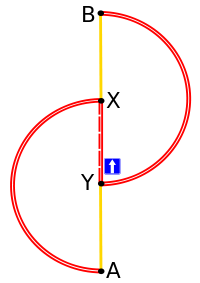
\includegraphics[width=0.7\textwidth]{img/braess2}
\caption{Uzupełniony układ drogowy}
\end{figure}
\end{minipage}\hfill
\begin{minipage}{.48\textwidth}
Do wyjściowego układu drogowego dodana zostaje autostrada:\\

YX, $t_{YX}(p) =  10 + p$ min\\

Aut jest nadal 6000 i wszystkie mają za zadanie przejechać trasę z A do B.

\end{minipage}\hfill
\end{frame}

\begin{frame}{Równowaga Nasha dla uzupełnionego układu\cite{braess}} 

Jeśli p, q i r to liczby aut w tysiącach pokonujących odpowiednio trasy AXB, AYB i AYXB, otrzymujmy równania:

\begin{center}
$p+q+r = 6 $\\
$t_{AX}(p)+t_{XB}(p+r) = t_{AY}(q+r) + t_{YB}(q) = t_{AY}(q+r)+t_{YX}(r)+t_{XB}(p+r)$
\newline\\
$50+p+10(p+r) = 10(q+r)+50+q = 10(q+r)+ 10 + r + 10(p+r)$
\end{center}
rozwiązaniem jest $p=q=r=2$.\\
Czas przejazdu każdej z tych dróg wynosi wówczas $50+2+10(2+2)=92$ minuty.
\end{frame}


\subsection{Słabe punkty istniejacych rozwiazań}
\begin{frame}{Słabe punkty istniejacych rozwiazań} 

Paradoks Braessa został sformułowany w roku 1970,
a od roku 1996 zaczęły pojawiać się prace negujące lub podważające paradoks\cite{newinsights}.
Wiele miast jednak brało i bierze pod uwagę paradoks Braessa podczas projektowania swojej przestrzeni:

\begin{itemize}
\item Korea, Seul, likwidacja m.in. estakad Cheonggyecheon,
\item Niemcy, Stuttgart, likwidacja dróg zbudowanych w latach 60,
\item USA, Nowy Jork, czasowe zamknięcie ulicy 42,
\item USA, Winnipeg.\cite{urban}
\end{itemize}  

\end{frame}


\section{Technologie i metody użyte}
\subsection{Symulator transportu}
\begin{frame}{Symulator transportu} 

	\begin{figure}[b]
	
\includegraphics[width=0.40\textwidth]{img/matsim}
	\caption{Logo symulatora transportu MATSim \cite{matsim}} 
	\end{figure}

\end{frame}

\subsection{Przestrzeń poszukiwań}
\begin{frame}{Przestrzeń poszukiwań} 
Najlepszego rozwiązania będę poszukiwał wykorzystując klasyczny algorytm genetyczny.

	\begin{figure}[b]
	
\includegraphics[width=0.40\textwidth]{img/math}
	\caption{Logo biblioteki Apache Commons Math \cite{math}} 
	\end{figure}

\end{frame}

\begin{frame}{Klasyczny algorytm genetyczny} 

\centering
\begin{minipage}[b]{.48\textwidth}
\begin{figure}[]
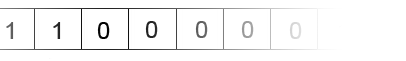
\includegraphics[width=\textwidth]{img/bool}
\caption{Fragment sieci w postaci tablicy binarnej }
\end{figure}
\end{minipage}\hfill
\begin{minipage}[b]{.48\textwidth}
\begin{figure}[]
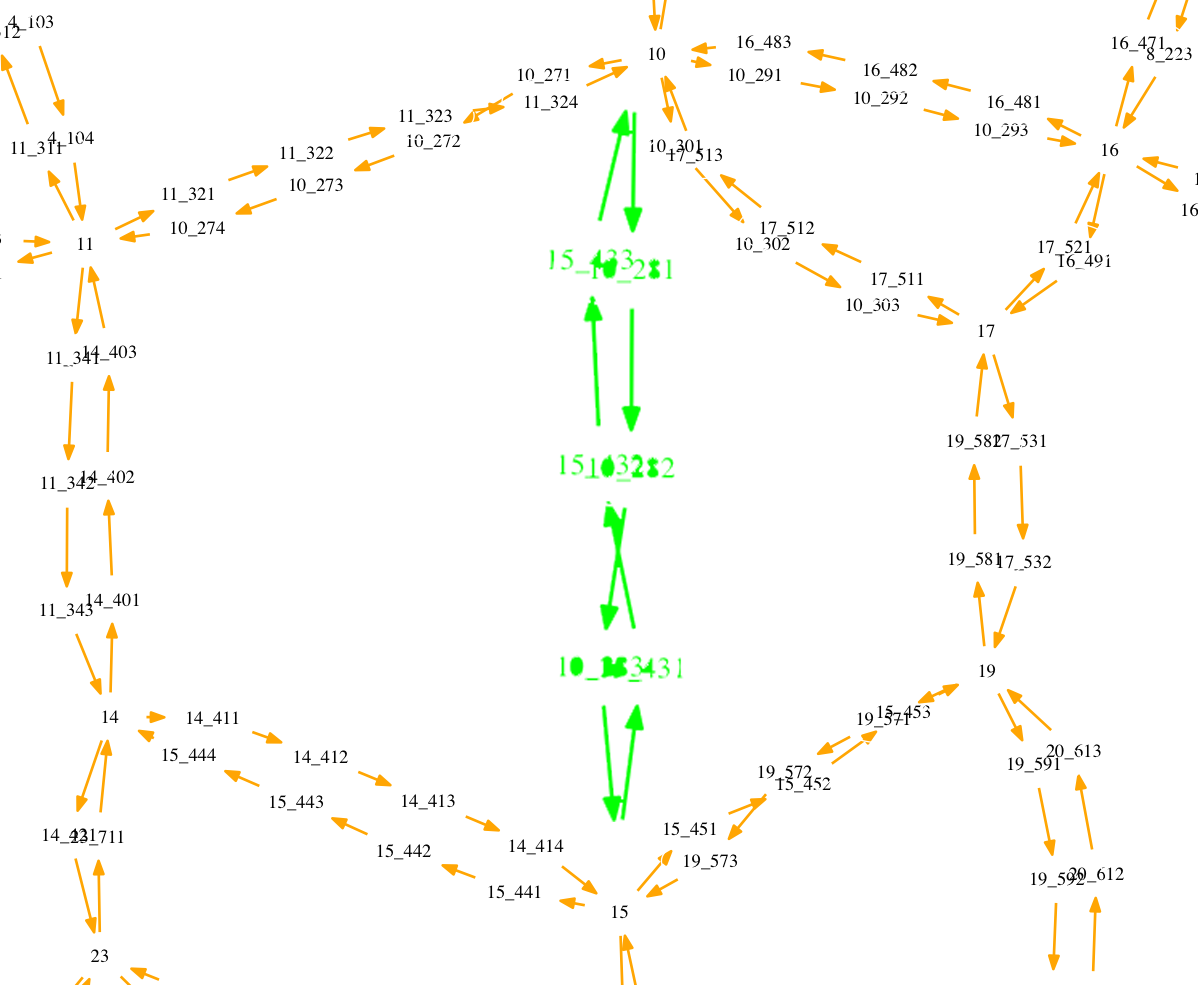
\includegraphics[width=\textwidth]{img/bool-efect}
\caption{Fragment sieci w postaci grafu}
\end{figure}
\end{minipage}\hfill

\end{frame}


\subsection{Technologie i metodologie programistyczne}
\begin{frame}{Technologie i metodologie programistyczne} 

\centering
\begin{minipage}[b]{.48\textwidth}

\begin{figure}

\includegraphics[width=0.7\textwidth]{img/java}
\caption{Logo Java\cite{java}}
\end{figure}
\begin{figure}

\includegraphics[width=0.7\textwidth]{img/eclipse}
\caption{Logo IDE Eclipse\cite{eclipse}}
\end{figure}

\end{minipage}\hfill
\begin{minipage}[b]{.48\textwidth}

\begin{figure}

\includegraphics[width=0.7\textwidth]{img/py}
\caption{Logo Python\cite{python}}
\end{figure}
\begin{figure}

\includegraphics[width=0.55\textwidth]{img/pydev}
\caption{Logo PyDev\cite{pydev}}
\end{figure}

\end{minipage}\hfill
\end{frame}

\section{Aplikacja}

\subsection{Dane wejściowe}
\begin{frame}{Dane wejściowe}

\lstset{
    language=xml,
    tabsize=3,
    rulesepcolor=\color{gray},
    keywordstyle=\color{blue}\bf,
    stringstyle=\color{red},
    breaklines=true,
    basicstyle=\ttfamily\scriptsize}
\lstinputlisting[language=Xml]{img/config.xml}

\end{frame}


\subsection{Wdrożenie}
\begin{frame}{Wdrożenie} 
\begin{figure}

\includegraphics[width=0.4\textwidth]{img/trisquel}
\caption{Logo Trisquel\cite{trisquel}}
\end{figure}
\end{frame}


\subsection{Przewidywane problemy}
\begin{frame}{Przewidywane problemy} 

\begin{itemize}
\item Brak gwarancji lepszego wyniku
\item Długi czas obliczeń
\item Duże wymagania dotyczące zasobów
\end{itemize}

\end{frame}


\section{Podsumowanie}

\subsection{Dyskusja wyników}
\begin{frame}{Natężenie ruchu}
\centering
\begin{minipage}[b]{.48\textwidth}
\begin{figure}[]
\includegraphics[width=0.7\textwidth]{{{img/s/graph6.00-7.00}}}
\caption{Ruch, 6.00-7.00, graf oryginalny}
\end{figure}
\end{minipage}\hfill
\begin{minipage}[b]{.48\textwidth}
\begin{figure}[]
\includegraphics[width=0.7\textwidth]{{{img/sc/graph6.00-7.00}}}
\caption{Ruch, 6.00-7.00, graf zmodyfikowany}
\end{figure}
\end{minipage}\hfill
\end{frame}

\begin{frame}{Natężenie ruchu}
\centering
\begin{minipage}[b]{.48\textwidth}
\begin{figure}[]
\includegraphics[width=0.7\textwidth]{{{img/s/graph7.00-8.00}}}
\caption{Ruch, 7.00-8.00, graf oryginalny}
\end{figure}
\end{minipage}\hfill
\begin{minipage}[b]{.48\textwidth}
\begin{figure}[]
\includegraphics[width=0.7\textwidth]{{{img/sc/graph7.00-8.00}}}
\caption{Ruch, 7.00-8.00, graf zmodyfikowany}
\end{figure}
\end{minipage}\hfill
\end{frame}

\begin{frame}{Natężenie ruchu}
\centering
\begin{minipage}[b]{.48\textwidth}
\begin{figure}[]
\includegraphics[width=0.7\textwidth]{{{img/s/graph8.00-9.00}}}
\caption{Ruch, 8.00-9.00, graf oryginalny}
\end{figure}
\end{minipage}\hfill
\begin{minipage}[b]{.48\textwidth}
\begin{figure}[]
\includegraphics[width=0.7\textwidth]{{{img/sc/graph8.00-9.00}}}
\caption{Ruch, 8.00-9.00, graf zmodyfikowany}
\end{figure}
\end{minipage}\hfill
\end{frame}

\begin{frame}{Natężenie ruchu}
\centering
\begin{minipage}[b]{.48\textwidth}
\begin{figure}[]
\includegraphics[width=0.7\textwidth]{{{img/s/graph15.00-16.00}}}
\caption{Ruch, 15.00-16.00, graf oryginalny}
\end{figure}
\end{minipage}\hfill
\begin{minipage}[b]{.48\textwidth}
\begin{figure}[]
\includegraphics[width=0.7\textwidth]{{{img/sc/graph15.00-16.00}}}
\caption{Ruch, 15.00-16.00, graf zmodyfikowany}
\end{figure}
\end{minipage}\hfill
\end{frame}

\begin{frame}{Natężenie ruchu}
\centering
\begin{minipage}[b]{.48\textwidth}
\begin{figure}[]
\includegraphics[width=0.7\textwidth]{{{img/s/graph16.00-17.00}}}
\caption{Ruch, 16.00-17.00, graf oryginalny}
\end{figure}
\end{minipage}\hfill
\begin{minipage}[b]{.48\textwidth}
\begin{figure}[]
\includegraphics[width=0.7\textwidth]{{{img/sc/graph16.00-17.00}}}
\caption{Ruch, 16.00-17.00, graf zmodyfikowany}
\end{figure}
\end{minipage}\hfill
\end{frame}

\begin{frame}{Natężenie ruchu}
\centering
\begin{minipage}[b]{.48\textwidth}
\begin{figure}[]
\includegraphics[width=0.7\textwidth]{{{img/s/graph17.00-18.00}}}
\caption{Ruch, 17.00-18.00, graf oryginalny}
\end{figure}
\end{minipage}\hfill
\begin{minipage}[b]{.48\textwidth}
\begin{figure}[]
\includegraphics[width=0.7\textwidth]{{{img/sc/graph17.00-18.00}}}
\caption{Ruch, 17.00-18.00, graf zmodyfikowany}
\end{figure}
\end{minipage}\hfill
\end{frame}

\begin{frame}{Natężenie ruchu}
\centering
\begin{minipage}[b]{.48\textwidth}
\begin{figure}[]
\includegraphics[width=0.7\textwidth]{{{img/s/graph18.00-19.00}}}
\caption{Ruch, 18.00-19.00, graf oryginalny}
\end{figure}
\end{minipage}\hfill
\begin{minipage}[b]{.48\textwidth}
\begin{figure}[]
\includegraphics[width=0.7\textwidth]{{{img/sc/graph18.00-19.00}}}
\caption{Ruch, 18.00-19.00, graf zmodyfikowany}
\end{figure}
\end{minipage}\hfill
\end{frame}

\begin{frame}{Wyniki agentów}
\centering
\begin{minipage}[b]{.48\textwidth}
\begin{figure}[]
\includegraphics[width=\textwidth]{{{img/s/scorestats}}}
\caption{Wyniki agentów, graf oryginalny}
\end{figure}
\end{minipage}\hfill
\begin{minipage}[b]{.48\textwidth}
\begin{figure}[]
\includegraphics[width=\textwidth]{{{img/sc/scorestats}}}
\caption{Wyniki agentów, graf zmodyfikowany}
\end{figure}
\end{minipage}\hfill
\end{frame}

\begin{frame}{Przebyta droga}
\centering
\begin{minipage}[b]{.48\textwidth}
\begin{figure}[]
\includegraphics[width=\textwidth]{{{img/s/traveldistancestats}}}
\caption{Przebyta droga, graf oryginalny}
\end{figure}
\end{minipage}\hfill
\begin{minipage}[b]{.48\textwidth}
\begin{figure}[]
\includegraphics[width=\textwidth]{{{img/sc/traveldistancestats}}}
\caption{Przebyta droga, graf zmodyfikowany}
\end{figure}
\end{minipage}\hfill
\end{frame}

\begin{frame}{Średni czas podróży}

Graf oryginalny: 1326.6473784330044 [sekund]\\
Graf zmodyfikowany: 1432.6902865295447 [sekund]\\

\vspace*{20px}
Wynik o $\approx 8 \%$ gorszy.

\end{frame}

\subsection{Perspektywy dalszych badań w dziedzinie}
\begin{frame}{Perspektywy dalszych badań w dziedzinie} 

\begin{figure}[h!]
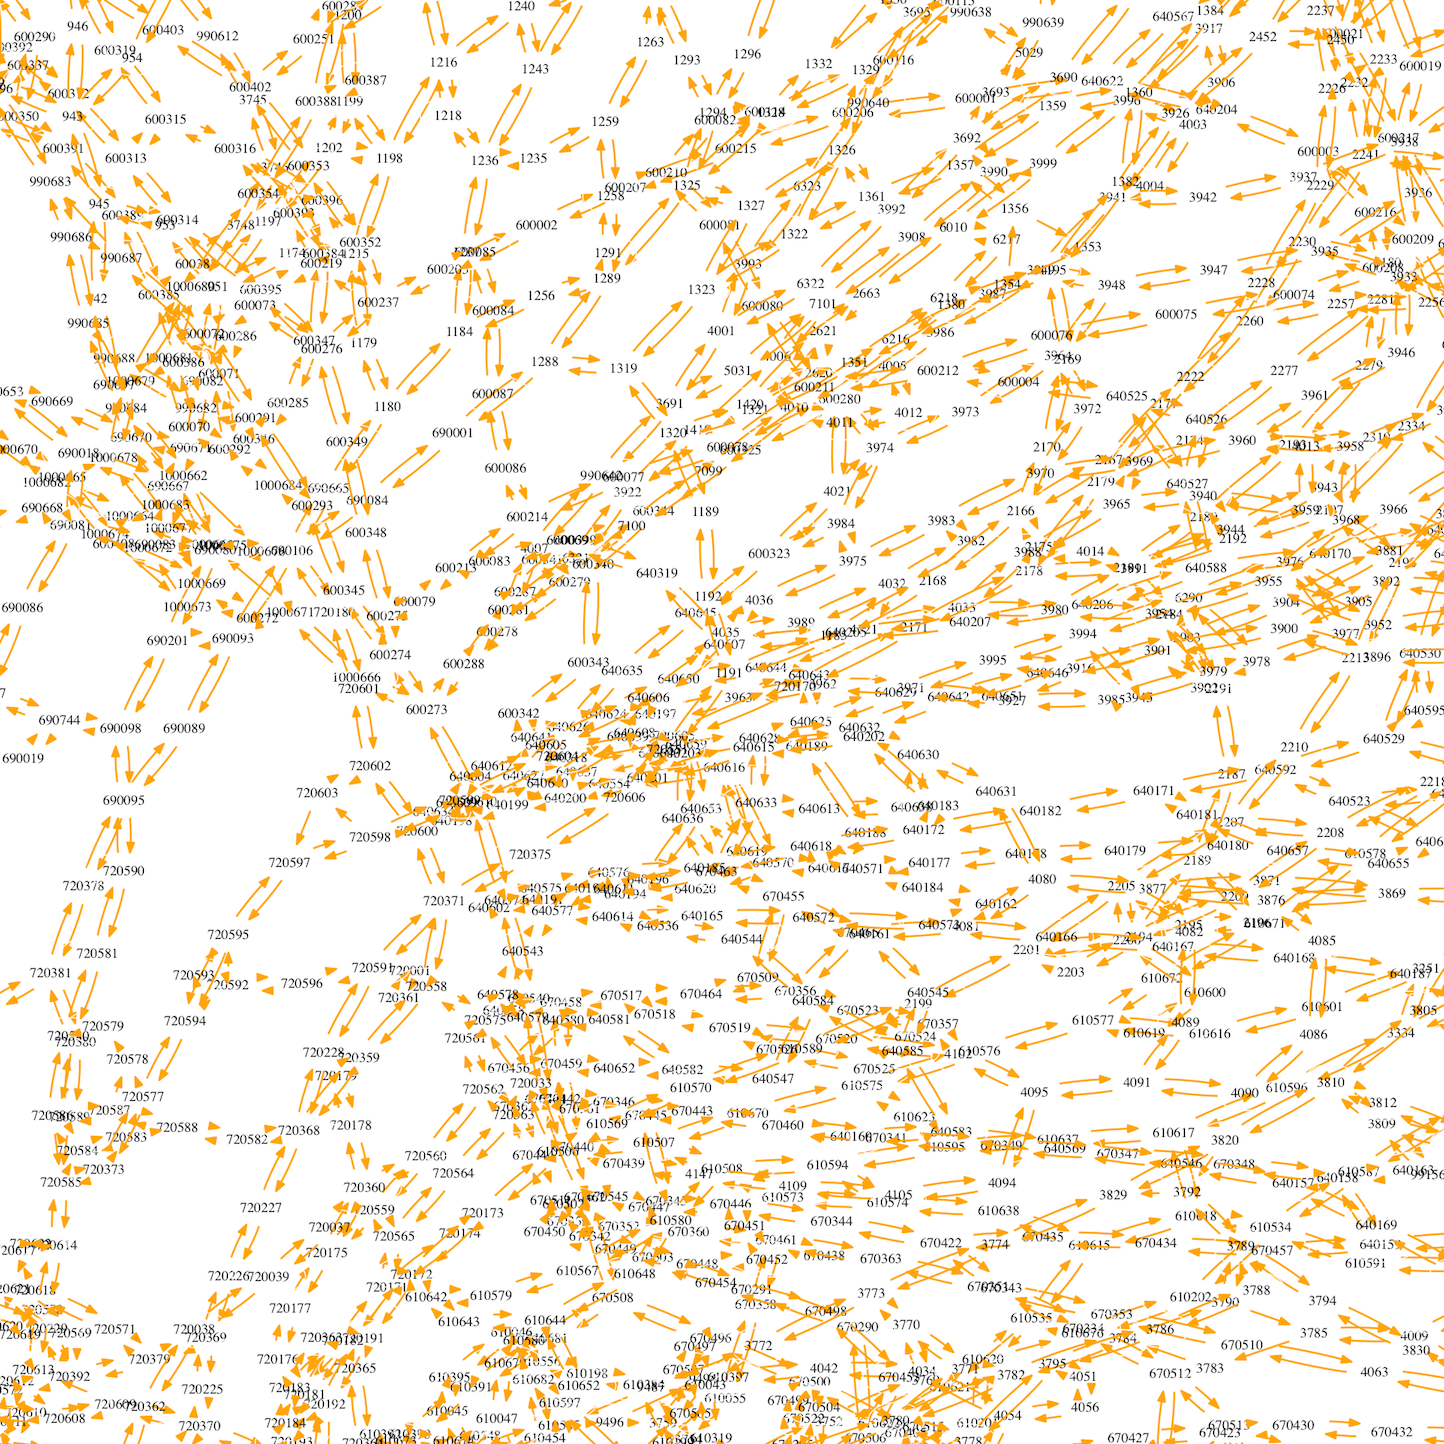
\includegraphics[width=0.50\textwidth]{img/berlin}
\caption{Część mapy Berlina}
\end{figure}

\end{frame}

\begin{frame}{Perspektywy dalszych badań w dziedzinie} 

\begin{figure}[h!]
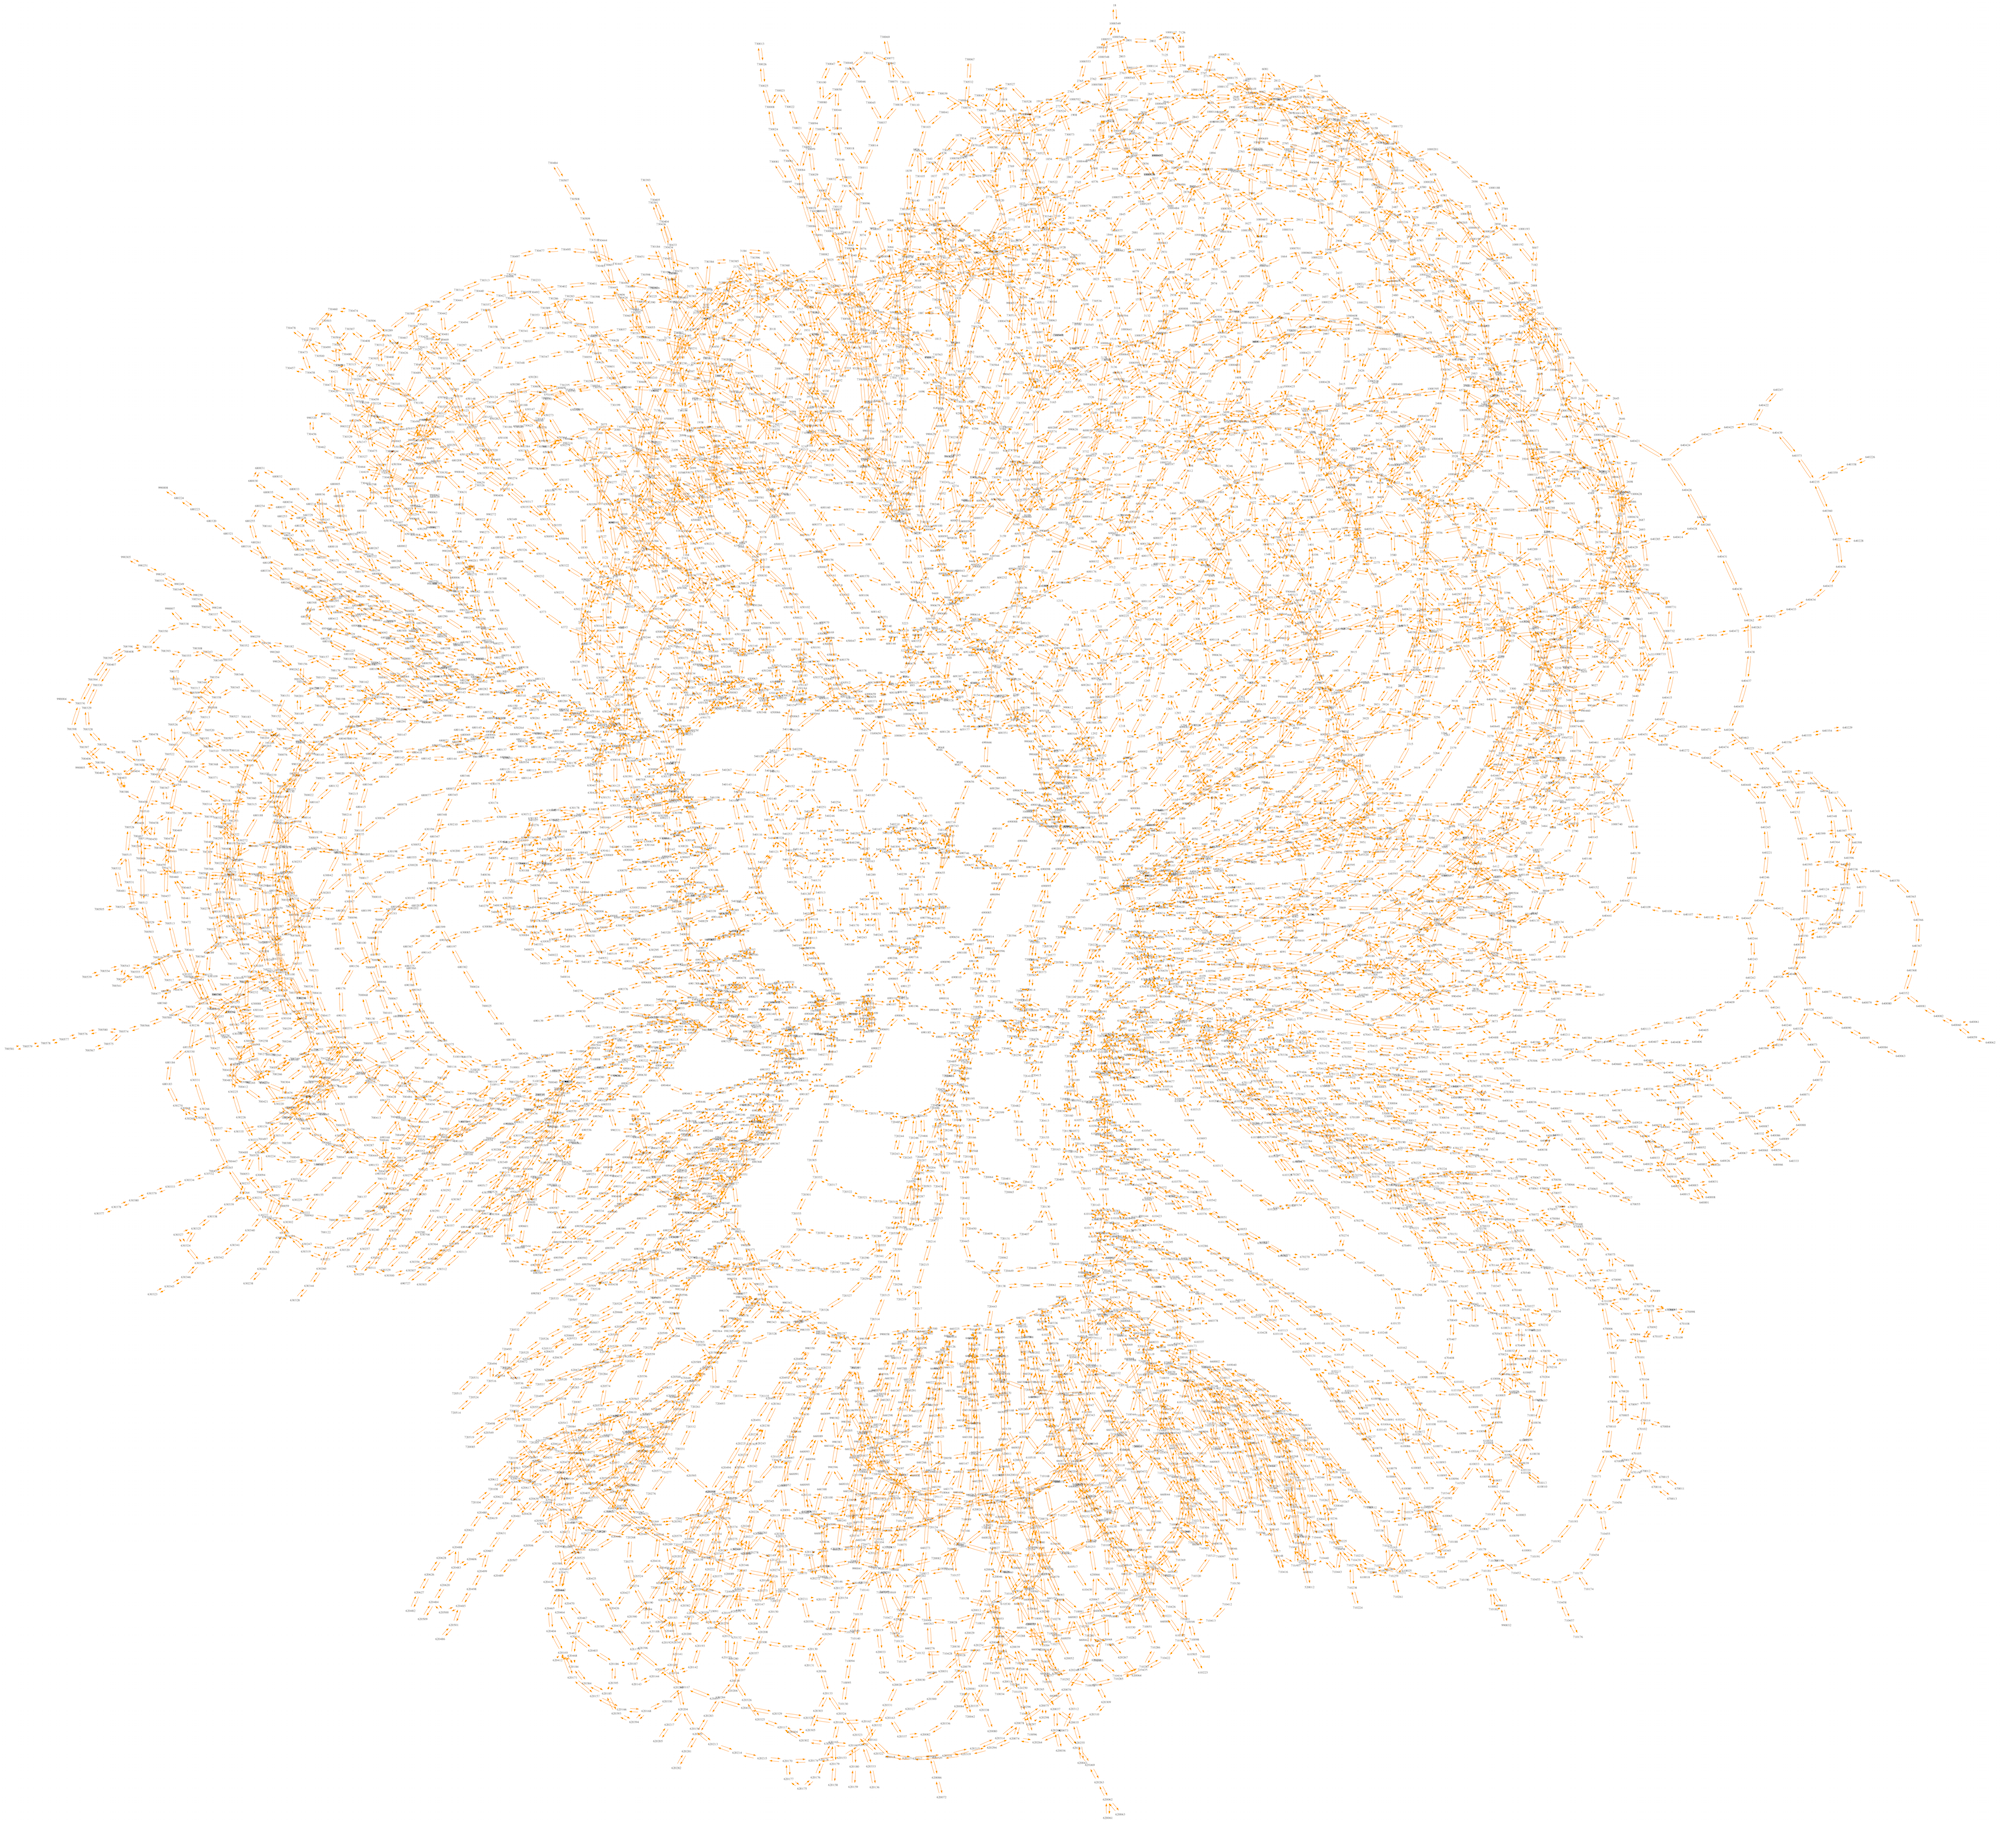
\includegraphics[width=0.55\textwidth]{img/berlin2}
\caption{Mapa Berlina}
\end{figure}

\end{frame}


\section{Bibliografia}
\begin{frame}[allowframebreaks]{Bibliografia}
\begin{thebibliography}{10}

\bibitem{investigation} 
	Leslie Arthur Keith Bloy, 
	\newblock \textit{An investigation into Braess’ paradox}, 02/2007

\bibitem{newinsights}
	Rric Pas and Shari Principio
	\newblock \textit{Braess’ paradox: Some new insights}, April 1996

\bibitem{conference} 
	Wataru Nanya, Hiroshi Kitada, Azusa Hara, Yukiko Wakita, Tatsuhiro Tamaki, and Eisuke Kita
	\newblock \textit{Road Network Optimization for Increasing Traffic Flow}
	\newblock Int. Conference on Simulation Technology, JSST 2013.

\bibitem{reducingtheeffects}
	Ana L. C. Bazzan and Franziska Klügl
	\newblock \textit{Reducing the Effects of the Braess Paradox with Information Manipulation}


\framebreak

\bibitem{matsim} 
	\url{http://matsim.org}	

\bibitem{math}
	\url{http://commons.apache.org/proper/commons-math}

\bibitem{java} 
	\url{http://www.java.com/pl/}

\bibitem{eclipse} 
	\url{https://eclipse.org}
				
\bibitem{python} 
	\url{http://pl.python.org}
	
\bibitem{pydev} 
	\url{http://pydev.org}
	
\bibitem{trisquel}
	\url{https://trisquel.info}
			

\framebreak

\bibitem{matsim-userg}
	M. Rieser, C. Dobler, T. Dubernet, D. Grether, A. Horni, G. Lammel, R. Waraich, M. Zilske, Kay W. Axhausen, Kai Nagel
	\newblock \textit{MATSim User Guide}
	\newblock updated September 12, 2014

\bibitem{siux}
	A. Chakirov
	\newblock \textit{Enriched Sioux Falls Scenario with Dynamic Demand}
	\newblock MATSim User Meeting, Zurich/Singapore, June 2013.
	
\bibitem{braess}
	\url{http://pl.wikipedia.org/wiki/Paradoks_Braessa}
	
\bibitem{urban}
	\url{http://urbnews.pl/paradoks-braessa/}
	

\end{thebibliography}
\end{frame}

\end{document}